\chapter{Data Collection}
\label{chap:data}

In Chapter~\ref{chap:intro}, I explained that a major motivation of this work is to investigate relatively low-resource mechanisms for content analysis that can help shift the focus of ICALL from form to meaning. In Chapter~\ref{chap:lit}, I examined related work in testing and ICALL. While numerous creative approaches to contextual content analysis are discussed in the literature, the data they rely on is typically not available to other researchers. With these considerations and the lessons learned from the dataset described in Chapter~\ref{chap:pilot} in mind, I decided to collect a corpus of picture description task responses for use in my experiments. I discuss the data collection instrument in Section~\ref{sec:pdt} and the participants in Section~\ref{sec:participants}. In Sections~\ref{sec:response-totals} and~\ref{sec:response-variation}, I present the total response counts for various categories and examine the variability of responses.


\section{Picture Description Task}
\label{sec:pdt}

%\subsection{PDT Stimuli}

The picture description task (PDT) is built around 30 images. Each image is a simple, cartoon-like vector graphic. These images were purchased from Shutterstock, a web-based graphics library\footnote{https://www.shutterstock.com/vectors}. In order to constrain response contents to the main action of each image, the images were modified to remove any non-essential detail or background; an example is shown in Figure~\ref{fig:image-prep}. Vector graphics are ideal for this use, because they tend to have an illustrational style with very little detail, as compared to photographs or drawings. Moreover, most consist of layers of graphic objects, and these objects can be easily moved, resized, deleted, combined or otherwise modified to compose the desired stimulus. More example images are presented in Figure~\ref{fig:example-pdt-items} and the full set is found in Appendix \ref{appendix:PDT_items}.

To factor out the influence of previous linguistic context, images are intentionally devoid of any text. In a few cases, symbols are used: two images have music notes; one displays a legible analog clock; one uses numerals in an arithmetic problem and one shows a question mark. The symbols were intended to elicit abstract concepts that are otherwise difficult to portray visually, like \textsc{teaching math} and \textsc{asking a question}. 

\begin{figure}[htb!]
\begin{center}
\begin{tabular}{|c|c|}
\hline
{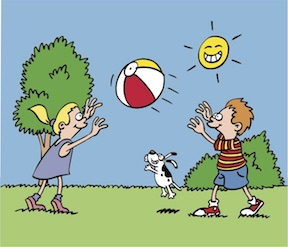
\includegraphics[width=0.38\columnwidth]{figures/throw-original.jpg}} & {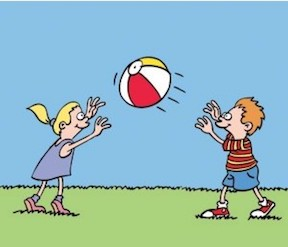
\includegraphics[width=0.38\columnwidth]{figures/I21cropped.jpg}} \\
\hline
Original image & Simplified PDT image \\
\hline
\end{tabular}
\caption{\label{fig:image-prep} All non-essential details were removed from the PDT images in order to focus participants' attention on the main action.}
\end{center}
\end{figure}

Each image was chosen for its depiction of an ongoing or imminent action (as opposed to a static image or ``still life'') performed by a person or an animal. The images are divided evenly into actions that are canonically intransitive, transitive or ditransitive in English. I chose these three categories because they indicate the number of actors and objects in a given event, and my approach to scoring responses should be able to handle this range of complexity. It should be noted that this categorization is imperfect, however, as some events in the PDT can be expressed in multiple ways, like \textit{The girl is riding a horse} (transitive construction) versus \textit{The girl is horseback riding} (intransitive construction). I attempted to minimize ambiguity (especially between intransitives and transitives) by avoiding images with possible light constructions, like \textit{He is taking a shower} versus \textit{He is showering}.


\begin{figure}[htb!]
%\begin{table}[t!] This line is giving me trouble when I go to typeset
\begin{center}
\begin{tabular}{|c|c|c|}
\hline
{
\includegraphics[width=0.29\columnwidth]{figures/I20.jpg}} & {
\includegraphics[width=0.3\columnwidth]{figures/I02.jpg}} & {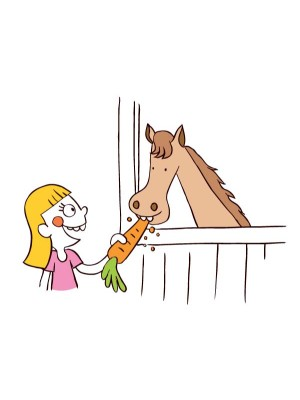
\includegraphics[width=0.3\columnwidth]{figures/I17.jpg}} \\
\hline
What is the girl doing? & What is the boy doing? & What is the girl doing? \\
\hline
\end{tabular}
\caption{\label{fig:example-pdt-items} PDT example images with their targeted questions. In the untargeted form, the question for each is \textit{What is happening?} From left to right, the examples represent one intransitive, transitive and ditransitive item.}
\end{center}
\end{figure}

Each PDT image is used in two different contexts: \textbf{targeted} and \textbf{untargeted}. An \textbf{item} consists of an image and a prompt question. For \textbf{targeted} items, questions take the form of \textit{What is $<$subject$>$ doing?}, with the subject provided (e.g., \textit{the girl}, \textit{the boy}; see Figure~\ref{fig:example-pdt-items}). For all \textbf{untargeted} items, the question is \textit{What is happening?}
%Thus, there are a total of 60 different items used in this study, with each of 30 images used once in a targeted prompt and once in an untargeted prompt.
Collecting these targeted and untargeted responses allows for the examination of response variation with and without a subject constraint. To elaborate, for targeted items, I expect less variation among responses; defining the subject in the prompt means all responses should reuse this subject and only vary in how they express the predicate. For untargeted items, some image prompts might allow for variation of the subject, however. For the image in Figure~\ref{fig:image-prep}, for example, valid responses could include \textit{The boy is throwing a ball to the girl} as well as \textit{The girl is catching a ball from the boy}. Understanding the effect of the subject constraint could help inform approaches to task design and automatic content assessment \citep{foster2009native, cho2013investigating}. 

Different participants performed different versions of the PDT, and multiple versions were necessary to collect roughly equal numbers of targeted and untargeted \textbf{responses} for each image. These versions vary in which images are presented as targeted items and which images are presented as untargeted items. Additionally, native speakers (NSs) were asked to provide two non-identical responses to each item (see Section~\ref{sec:participants}), but non-native speakers (NNSs) were asked to provide only one response per item, so different PDT versions were used for these groups. The PDTs were hosted online via Survey Monkey\footnote{https://www.surveymonkey.com}, and all participants submitted their responses through this platform. %Survey Monkey restricts the number of questions included in surveys used for purchasing crowdsourced responses, so the PDTs were split accordingly for this group.

In each (full-length) PDT, targeted items are presented in the first half, and untargeted items are presented in the second half. This targeted-untargeted ordering is intended to avoid the possibility that in an untargeted-targeted task, respondents might notice that the question for each untargeted item is always the same in the first half and finish the task hastily without noticing that later targeted items specify the subject. Each half is introduced with instructions, including an example item with sample responses. The instructions ask participants to focus on the main event depicted in the image and for each response to be one complete sentence. Because the PDT was presented as an online survey, all participants typed their responses. Participants were instructed not to use any reference materials, but browser-based spell checking was not disabled, and participants are assumed to have used it as necessary.

The main task instructions are presented in (\ref{exe:pdt-instructions-a}). Additional instructions provided to NSs are presented in (\ref{exe:pdt-instructions-b}). The full set of PDT versions is available for download with the SAILS Corpus.\footnote{https://github.com/sailscorpus/sails}

\begin{exe}
  \ex\label{exe:pdt-instructions-a}\textbf{Instructions:} In this task, you will view a set of images. For each image, please write \textbf{one sentence} to answer the question provided with the image. It is important to write a \textbf{complete sentence}, not a word or phrase.
\end{exe}

\begin{exe}
  \ex\label{exe:pdt-instructions-b}\textbf{Additional Instructions for NSs:} Then, you will be asked to write a second, \textit{different} answer, which is also a complete sentence. This might involve rewording or reorganizing your first sentence. It does not need to be \textit{completely} different; some words may be the same. If you cannot think of another way to answer the question, you may leave the second answer space empty, but any second responses you provide will be greatly appreciated.
\end{exe}

\section{Participants}
\label{sec:participants}

This study involved a total of 499 PDT participants. Of these, 141 were NNSs, recruited from intermediate and advanced writing courses in the English Language Improvement Program at Indiana University. These participants performed the task in a computer lab with a researcher present. They were native speakers of Mandarin Chinese (125), Korean (4), Burmese (3), Hindi (2), and one native speaker each of Arabic, Indonesian Bahasa, German, Gujarati, Spanish, Thai and Vietnamese. Because nearly 90\% of these recruits were native speakers of Chinese, care should be taken when drawing conclusions from the corpus; patterns observed among the NNSs here might not apply broadly to all NNSs.

Responses from 329 of the NSs were purchased via Survey Monkey, where survey takers can earn credits that they can redeem for prizes or convert to donations to charities. Asking NSs to provide two responses doubles the length of the survey, exceeding the platform's limits on survey length for purchases responses, so the task was divided into two separate surveys for NSs. Thus while each NS and NNS provided 30 responses, each NNS responded to all 30 PDT items while each NS responded to only 15.

The remaining 29 NS participants were people known to me personally. Due to this relatively small number of participants, their data was not used for modeling or evaluating NNS responses, but it was annotated and is included in the SAILS Corpus. Unless specifically noted otherwise, the NS data discussed throughout this dissertation is the crowdsourced data. Where relevant, however, I refer to these two groups as the \textbf{Familiar Native Speakers (FNSs)} and the \textbf{Crowdsourced Native Speakers (CNSs)}. Future work should include collecting much more FNS data and comparison of the two groups to better understand the differences in quality, as CNSs are almost certainly less likely to perform the task in good faith.

All participants completed a background questionnaire at the beginning of the PDT. This included questions about first and second languages, gender, age, national origin, amount of English language instruction and length of residency in English-speaking locations. This questionnaire is included as part of the PDT, and the background information provided by participants is included in the SAILS Corpus files. A summary of some of the demographic information is shown in Table~\ref{tab:demographics}.

\begin{table}[htb!]
\begin{center}
\begin{tabular}{|l|rr|rr|rr|}
\hline
& \multicolumn{2}{|c|}{NNS} & \multicolumn{2}{|c|}{CNS} & \multicolumn{2}{|c|}{FNS} \\
\hline
\hline
Mean age & \multicolumn{2}{|r|}{18.7} & \multicolumn{2}{|r|}{45.0} & \multicolumn{2}{|r|}{39.1} \\
\hline
Median age & \multicolumn{2}{|r|}{18.0} & \multicolumn{2}{|r|}{44.0} & \multicolumn{2}{|r|}{35.0} \\
\hline
\hline
Male & 56 & (39.7\%) & 138 & (41.9\%) & 17 & (58.8\%) \\
\hline
Female & 76 & (53.2\%) & 172 & (52.3\%) & 11 & (37.9\%) \\
\hline
Unknown & 9 & (6.4\%) & 19 & (5.8\%) & 1 & (3.4\%) \\
\hline
\end{tabular}
\caption{\label{tab:demographics} Age and gender information for the three participant groups (Non Native Speakers, Crowdsourced Native Speakers and Familiar Native Speakers).}
\end{center}
\end{table}
%& \multicolumn{3}{|c|}{Response Counts} \\


In previous similar work \citep{king:dickinson:13},
%\citep{king:dickinson:13,king:dickinson:16},
NSs were found to produce less variation than NNSs. Many NSs provided identical responses or responses that hew very closely to the most canonical way of expressing the main action. A major motivation for collecting the current corpus was the notion of assessing NNS response content by comparing it against the NS responses. Among other things, this involves the matching of words or syntactic dependencies and thus benefits from a broad set of acceptable responses in the gold standard. For this reason, NSs were asked to provide two non-identical responses, in the hopes that this would result in a wide range of examples of native-like responses for the NNS responses to be compared against.

\section{Response Totals}
\label{sec:response-totals}

A total of 13,533 responses were collected. The response counts for each participant group are presented in Table~\ref{tab:response-counts}. Including the second responses collected from NSs, roughly two thirds of the corpus come from the NS groups. The overwhelming majority of responses appear to be given in good faith, but a small number of responses (primarily from the CNS group) are problematic in this regard, as shown in Table~\ref{tab:bad-faith}. These may contain gibberish or obscenities or are otherwise inappropriate for the task. Such responses would also be expected in an ICALL environment, so they were not removed from the corpus. Instead, these responses were simply annotated like all others (see Chapter~\ref{chap:annotation}). Indeed, automatically assigning low scores to inappropriate responses is a central challenge and goal in this project (see Chapter \ref{chap:optimization}).

\begin{table}[htb!]
\begin{center}
\begin{tabular}{|l||r|r||r|}
\hline
& \multicolumn{3}{c|}{Response Counts} \\
\hline
 Group & First & Second & Total \\
\hline
\hline
NNS & 4290 & 0 & 4290 \\
\hline
\hline
NS (all) & 4634 & 4609 & 9243 \\ %%LK: Yes, 0.949 is correct in both cases here
\hline
\multicolumn{1}{|r||}{FNS} & 642 & 641 & 1283 \\ 
\hline
\multicolumn{1}{|r||}{CNS} & 3992 & 3968 & 7960 \\
\hline
\hline
Total & 8924 & 4609 & 13,533 \\
\hline
\end{tabular}
\caption{\label{tab:response-counts} First and second response counts for the SAILS Corpus participant groups. Familiar (FNS) and crowdsourced (CNS) are subgroups of NS. NNS participants are not asked to provide a second response.}
\end{center}
\end{table}

\begin{table}[htb!]
\begin{center}
\begin{tabular}{|l|}
\hline
Exemplar: \textit{The girl is laughing.} \\
\hline
Girl ate a 2x4 and is vomiting toothpicks. \\
\hline
I have to poop so bad. \\
\hline
\hline
Exemplar: \textit{The boy is eating pizza.} \\
\hline
How is the pizza staying perfectly horizontal when the boy is holding it so close to the tip? \\
\hline
see my last statement \\
\hline
\hline
Exemplar: \textit{The girl is feeding a carrot to a horse.} \\
\hline
Creepy clown child grinding her carrot down on poor Ed's beaver teeth \\
\hline
Hoj \\
\hline
%Hey man \\
%\hline
\end{tabular}
\caption{\label{tab:bad-faith} Crowdsourced responses for the items shown in Figure~\ref{fig:example-pdt-items}, showing one exemplar response and two examples of problematic or bad faith responses for each item.}
\end{center}
\end{table}


\section{Response Variation}
\label{sec:response-variation}
Type-to-token ratios (TTR) are commonly used as an indication of how varied or homogenous a set of data is. This number ranges between 0 and 1. In a set of data where most instances or \textit{tokens} are unique (\textit{types}), the number of types per tokens approaches 1. In a set of data where most tokens are identical, the number of types per tokens approaches 0. With regard to language data, TTRs are often used on the word level, to calculate the lexical density of a document, for example \citep{granger2002computer}. In this case, however, I calculated type-to-token ratios (TTRs) on the response level for the entire set of items. For this calculation, final punctuation was ignored, and all responses were converted to lowercase. To illustrate, the first three response \textit{tokens} in Table~\ref{tab:type-token-examples} would constitute a single response \textit{type}.

\begin{table}[htb!]
\begin{center}
\begin{tabular}{|l|l|l|}
\hline
Types & Tokens & Response \\
\hline
1 & 1 & The woman is holding a dog \\
\hline
1 & 2 & the woman is holding a dog! \\
\hline
1 & 3 & The Woman is holding a Dog. \\
\hline
2 & 4 & The woman is hugging a puppy. \\
\hline
3 & 5 & The woman squeezed a dog. \\
\hline
\end{tabular}
\caption{\label{tab:type-token-examples} This toy dataset shows how TTR is calculated on the response (sentence) level. Ignoring punctuation and capitalization, the first three response tokens here constitute a single response type. The TTR for this set would be 3:5, or 0.6.}
\end{center}
\end{table}

%\begin{exe}[h!]
%  \ex\label{exe:ttr-1}The woman is holding a dog
%\end{exe}
%\begin{exe}[h!]
%  \ex\label{exe:ttr-2}the woman is holding a dog!
%\end{exe}
%\begin{exe}[h!]
%  \ex\label{exe:ttr-3}The Woman is holding a Dog.
%\end{exe}

The TTRs for the corpus are presented in Table~\ref{tab:ttr}. 
For each cell in this table, the corpus contains 10 items, for each of which there are roughly 150 NS responses and 70 NNS responses. 
TTR is highly sensitive to text length, so to control for the imbalance between NS and NNS responses, the TTR was calculated for each item and each group (NS and NNS) based on a random sample of 50 responses \citep{grieve2007}.  This was repeated 10 times and then averaged to produce a final TTR for each item. These item TTRs were then averaged as intransitives, transitives and ditransitives. The ratios show the direct relationship between the complexity of the event portrayed (represented here as intransitive, transitive and ditransitive) and the degree of variation elicited. In all cases, TTR increases with this complexity.
%Interestingly, this trend seems more pronounced in the NNS responses; in the targeted NNS responses, the TTRs for intransitive and ditransitive items are 0.381 and 0.817, respectively, compared to 0.628 and 0.835 for NS responses. \textbf{*Might this be explained by the inclusion of NNS 2nd responses? Let's investigate*}\lk{1st vs 2nd?} 
The ratios also show that in all cases, as expected, variation is greater for untargeted items than it is for targeted items. In other words, asking about a particular subject in the prompt question does constrain the variety of responses, as expected.

\begin{table}[h!]
\begin{center}
\begin{tabular}{|l||l|l||l|l|}
\hline
 & \multicolumn{2}{|c||}{Targeted} & \multicolumn{2}{|c|}{Untargeted} \\
\hline
 Set & NS & NNS & NS & NNS \\
\hline
\hline
Intrans & 0.628 & 0.381 & 0.782 & 0.492 \\
\hline
Trans & 0.752 & 0.655 & 0.859 & 0.779 \\ %%LK: Yes, 0.949 is correct in both cases here
\hline
Ditrans & 0.835 & 0.817 & 0.942 & 0.936 \\ 
\hline
\end{tabular}
\caption{\label{tab:ttr} NS and NNS type-to-token ratios (TTR) for complete responses (not words), for the full corpus.}
\end{center}
\end{table}

Additionally, from Table~\ref{tab:ttr} we can see that the NS set contains a greater degree of response variation than does the NNS set. Note that the TTRs here are calculated on \textit{all} responses, and the NS participants each provided two responses per item, whereas the NNS participants were only asked to provide one response per item. This suggests that asking for two responses is an effective way of collecting a broader range of NS responses. This variability can be more closely examined in Table~\ref{tab:ttr1v2}, which presents separate TTRs for all NS participants' first responses and second responses. The numbers show that in general, first responses are far less varied than second responses. As we can see, among first responses, variability increases along with item complexity. The pattern holds for targeted second responses, although it is not as pronounced. For untargeted second responses, this monotonic increase in variability is not present, but all three TTRs vary by less than three percent, indicating that a ceiling effect is at work. In other words, untargeted second responses are unconstrained by the task to such an extent that even the least complex responses---the intransitives---approach a level of variation roughly equal to the more complex transitive and ditransitive responses.

Finally, for ease of comparison, Table~\ref{tab:ttr1v1} presents the (NS only) first response TTRs from Table~\ref{tab:ttr1v2} alongside the NNS first (and only) response TTRs from Table~\ref{tab:ttr}. These comparisons should be made with caution, however, as they cannot account for the possibility of task effects arising from the different instructions given to NS and NNS participants. In other words, it is possible that the anticipation of providing a second response influences a NS participant's choice of first response, and any such effect would be absent for NNS participants. A future study in which NSs are asked to provide only one response per item could be useful in examining the possibility of such a task effect. As it stands, the table suggests that NNSs generally do exhibit greater response variability than NSs; the only exception to this trend appears among the intransitive untargeted items. This trend is in keeping with the observations from previous work \citep{king:dickinson:13}, which found that NSs tend toward canonical forms, while NNSs use whatever language may be available to them, resulting in greater variation. As described above, this was the motivation for asking NSs for two responses.

\begin{table}[h!]
\begin{center}
\begin{tabular}{|l||l|l||l|l|}
\hline
 & \multicolumn{2}{|c||}{Targeted} & \multicolumn{2}{|c|}{Untargeted} \\
\hline
 Set & R1 & R2 & R1 & R2 \\
\hline
\hline
Intrans & 0.343 & 0.819 & 0.549 & 0.939 \\
\hline
Trans & 0.509 & 0.895 & 0.682 & 0.926 \\ %%LK: Yes, 0.949 is correct in both cases here
\hline
Ditrans & 0.641 & 0.948 & 0.864 & 0.955  \\ 
\hline
\end{tabular}
\caption{\label{tab:ttr1v2} TTRs for complete responses, separated by first responses (R1) and second responses (R2). The ratios here are calculated from all NS responses; NNS responses are not included.}
\end{center}
\end{table}

\begin{table}[h!]
\begin{center}
\begin{tabular}{|l||l|l||l|l|}
\hline
 & \multicolumn{2}{|c||}{Targeted} & \multicolumn{2}{|c|}{Untargeted} \\
\hline
 Set & NS & NNS & NS & NNS \\
\hline
\hline
Intrans & 0.343 & 0.381 & 0.549 & 0.492 \\
\hline
Trans & 0.509 & 0.655 & 0.682 & 0.779 \\ %%LK: Yes, 0.949 is correct in both cases here
\hline
Ditrans & 0.641 & 0.817 & 0.864 & 0.936  \\ 
\hline
\end{tabular}
\caption{\label{tab:ttr1v1} TTRs for complete responses, comparing first responses only.}
\end{center}
\end{table}

Having examined response variation in a rather abstract sense here, Chapter~\ref{chap:annotation} will focus on annotating response features to obtain a more fine-grained view of the ways in which responses can vary.

